\documentclass[11pt]{beamer}
\usetheme{Warsaw}
\usepackage[T1]{fontenc}
\usepackage[utf8]{inputenc}
\usepackage{amsmath}
\usepackage{amsfonts}
\usepackage{amssymb}
\usepackage{graphicx}
\graphicspath{{imgs/}}
\usepackage{setspace}
\usepackage{hyperref}



\author{Chen ZHANG \inst{1,2}}
\title{Slide Template}
%\setbeamercovered{transparent} 
%\setbeamertemplate{navigation symbols}{} 
\setbeamertemplate{enumerate items}[default]


\logo{
\includegraphics[width=.25\textwidth]{logo.jpg}}

\institute[UNI]{\inst{1}Institute 1, \inst{2}Institute 2 $@$ Shenzhen, China\\[2.5ex] {Git URL: \href{https://github.com/CubicZebra/}{\color{cyan}\underline{CubicZebra}}}}

\date{}


%\subject{} 
\newcommand{\code}[1]{\texttt{#1}}
\AtEndDocument{\begin{frame}{\huge \quad Thanks for your attention.}\end{frame}}


\begin{document}

\begin{frame}
\titlepage
\end{frame}

\begin{frame}
\tableofcontents
\end{frame}

\section{Section 1}
\subsection{subsection 1.1}
\begin{frame}{items and code}
\begin{enumerate}
	\item text item 1:
    \begin{enumerate}
    	\item something about item 1
        \item another thing about item 1
    \end{enumerate}
    \item code item 2:
    \begin{enumerate}
    	\item can use code like: \code{conda activate env}
        \item or multi-lines: \\
        \code{for s in "Hello World":}\\
        \qquad \code{print(s)}
    \end{enumerate}
\end{enumerate}
\end{frame}

\subsection{subsection 1.2}
\begin{frame}{layout and style}
    \begin{minipage}[t]{0.5\textwidth}
        \vspace{0pt}
        \begin{itemize}
            \item emphasis \emph{one} and \emph{two}
            \item customize  via \emph{\color{red}three} syntax
            \item code \code{rm} is dangerous $\rightarrow$ \\ {\footnotesize\color{olive}(*more flexible \code{customize} and figure insert)}
        \end{itemize}
    \end{minipage}%
    \hfill
    \begin{minipage}[t]{0.45\textwidth}
        \vspace{0pt}
        \centering
              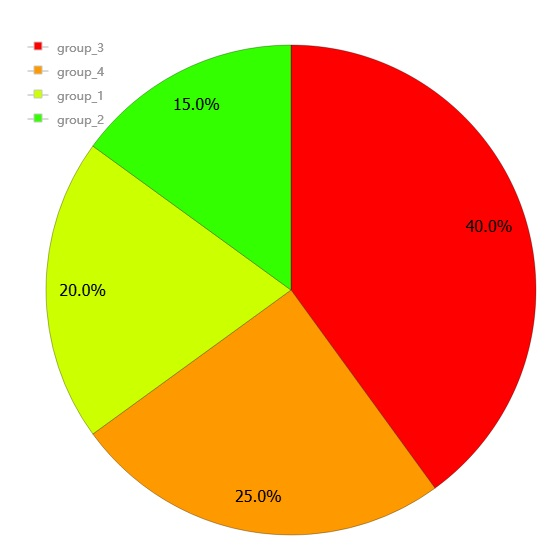
\includegraphics[height=5cm, width=4.5cm]{fig1.jpg}
    \end{minipage}
\end{frame}

\section{Section 2}
\subsection{subsection 2.1}
\begin{frame}[t]{another layout}
	\begin{minipage}[t]{1\textwidth}
        \vspace{0pt}
        \begin{itemize}
            \item {try vertical view like:}\\
            \singlespacing
            \centering
            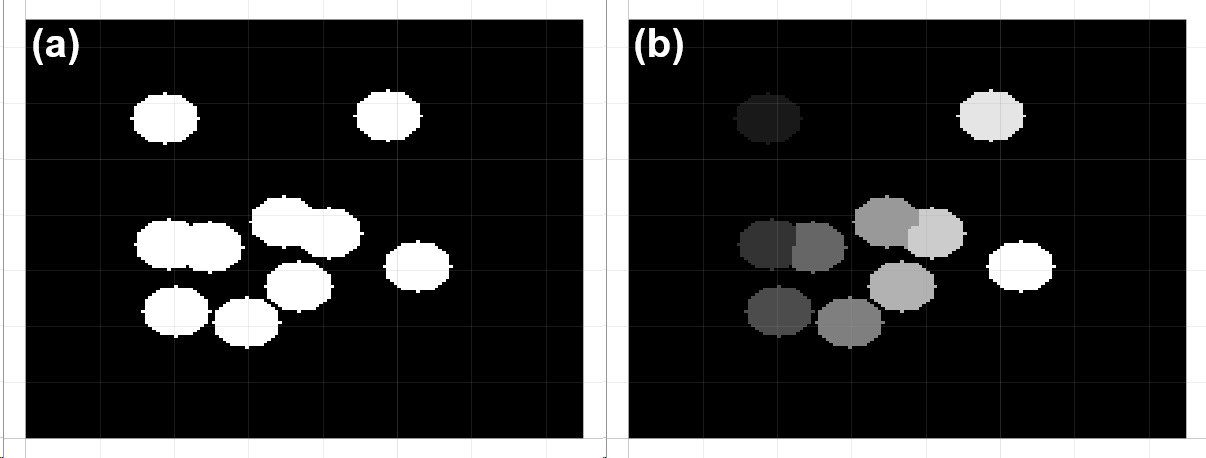
\includegraphics[scale=0.5]{fig2.jpg}
        \end{itemize}
    \end{minipage}%
\end{frame}


\subsection{subsection 2.2}
\begin{frame}{some math expression}
	\begin{enumerate}
		\item for plain: \\ $\because m \in (0, 1] \therefore \eta = 2m/(1+m) \in (0, 1]$
		\item for bold: \\ $\boldsymbol{X} = \boldsymbol{uu}^T$
	\end{enumerate}
\end{frame}

\end{document}